\chapter{\label{ch:simu_resp_mus}Respiratory Muscles Simulation}
As seen in chapter \ref{ch:human_torso_model}, section \ref{sec:breathing_mechanisms}, breathing can be split into two different mechanisms: rib cage breathing and abdominal breathing. This chapter describes the muscle element model we used and explains in detail the muscles responsible for these two breathing mechanisms and their actions. Finally, it details how these muscles are simulated and activated in the model.

% -------------------------------------------------------------
% Section
% -------------------------------------------------------------
\section{\label{sec:spring_muscle_element}Spring muscle element}
The human body is put into motion by the activation of muscles linking its different components. According to Zajac \cite{zajac1989muscle}, there are two fundamental assumptions about real muscles:
\begin{enumerate}
	\item A muscle can contract but not expand actively. In addition, it cannot generate force outside of its operating length range.
	\item A muscle contains a damping factor which makes it resist contraction based on the speed of shortening.
\end{enumerate}

Given these constraints, we modelled each muscle we used as a spring and a damper in parallel linking \emph{nodal masses} which are in our case the different bones (this model was used and validated by Grzeszczuk and Terzopoulos \cite{grzeszczuk1995automated}). The dynamics of our biomechanical model is specified by the equations of motion (termed `Lagrangian equations of motion' in \cite{grzeszczuk1995automated}): 

\begin{equation} \label{eq:lagrangian} m_{i} \ddot{\mathbf{x}}_{i} + \gamma_{i} \dot{\mathbf{x}}_{i} + \displaystyle\sum\limits_{j \in N_{i}} \mathbf{f}_{ij}^s = \mathbf{f}_{i} \end{equation}

where node  $ i $ has mass $ m_{i} $, position $ \mathbf{x}_{i}(t) = [x_{i}(t), y_{i}(t), z_{i}(t)] $, velocity $ \dot{\mathbf{x}}_{i} $, acceleration $ \ddot{\mathbf{x}}_{i} $, damping factor $ \gamma_{i} $ and where $ \mathbf{f}_{i} $ is an external force. $ N_{i} $ is the set of nodes connected to node $ i $. The spring $ S_{ij} $, which connects node $ i $ to neighbouring nodes $ j \in N_{i} $, exerts the force $ \mathbf{f}_{ij}^s $ on node $ i $ and $ - \mathbf{f}_{ij}^s $ on node $ j $:

\begin{equation} \label{eq:spring_muscle} \mathbf{f}_{ij}^s = -( c_{ij} e_{ij} + \gamma_{ij} \dot{e}_{ij} ) \frac{\mathbf{r}_{ij}}{\lVert \mathbf{r}_{ij} \rVert} \end{equation}

where $ c_{ij} $ is the stiffness gain, $ \gamma_{ij} $ is the damping gain and $ e_{ij}(t) = \lVert \mathbf{r}_{ij} \rVert - l_{ij} $ is the deformation of the spring with separation vector $ \mathbf{r}_{ij}(t) = \mathbf{x}_{j} - \mathbf{x}_{i} $. The rest length of the spring is $ l_{ij} $.

For rigid bodies (bones) in our 3D model, we use a rigid solver node to calculate dynamics and move each vertex according to the laws of physics. This node is called the \emph{rigid solver} as detailed in \cite{jameson1981numerical}, which solves the differential equations of the dynamics via the Runge Kutta Adaptive method, which, in comparison to the Mid-Point and Runge Kutta methods, provides greater accuracy.

% -------------------------------------------------------------
% Section
% -------------------------------------------------------------
\section{\label{sec:rib_cage}Rib cage}
During breathing, the rib cage is put into motion via several muscles connected to the ribs, namely the intercostals and the scalene muscles (also called the accessory inspiratory muscles).

\subsection{\label{subsec:intercostal_mus}Intercostal muscles}
Intercostal muscles, composed of the external and the internal intercostals, are two thin muscle layers occupying the space between two ribs as shown in figure \ref{fig:gray_stud_intercostals}. The intercostal spaces contain two layers of intercostal muscle in their lateral portion but they contain a single layer in their ventral and dorsal portions: ventrally between the sternum and the chondrocostal junctions there are only internal intercostals called the `parasternal intercostal muscles', dorsally from the angles of the ribs to the vertebrae there are only external intercostals. The external intercostal muscles have the greatest inspiratory moment in the dorsal portion of the rib cage. Experimentally, inspiratory activity in the external intercostals is highest in the dorsal area and declines gradually in the caudal and ventral directions. External intercostal muscles contract together during inspiration. Conversely, the internal intercostal muscles have the greatest inspiratory moment in the ventral area and are only active during expiration. The topographic distribution of expiratory activity in these muscles mirrors the topographic distribution of expiratory effect (see figure \ref{fig:curvature_rib}).

\begin{figure}
	\centering
	 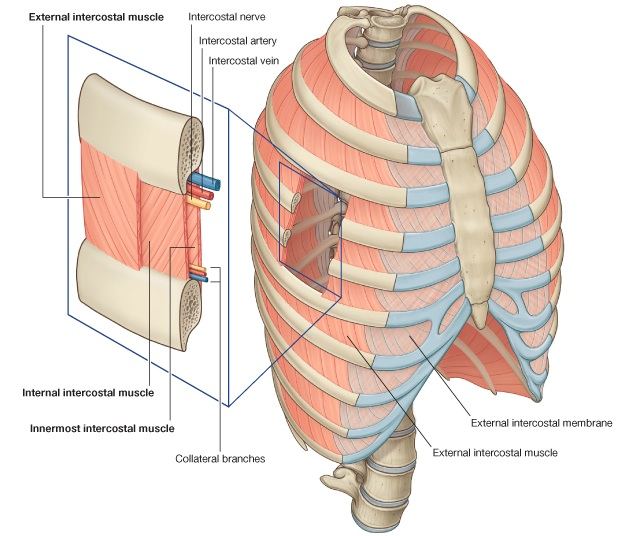
\includegraphics[scale=0.6]{pics/gray_stud_intercostals.jpg}
	\caption[Intercostal muscles]{\label{fig:gray_stud_intercostals}Intercostal muscles. Diagram taken from \cite{drake2005gray}.}	
\end{figure}

\begin{figure}
	\centering
	 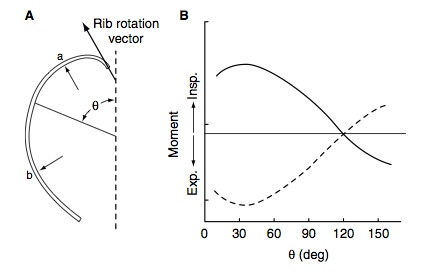
\includegraphics[scale=0.6]{pics/curvature_rib.jpg}
	\caption[Effects of rib curvature on the net moment exerted by an intercostal muscle]{\label{fig:curvature_rib}Effects of rib curvature (B) on the net moment exerted by an intercostal muscle located by the angle $\Theta$ (A). The external intercostal muscle (continuous line) has the greatest inspiratory moment in the dorsal portion of the rib cage ($\Theta$ between 15~$^\circ$ and 60~$^\circ$), this moment decreases and reverses into an expiratory moment for $\Theta \geq 120~^\circ$. The internal intercostal muscle moment (dashed line) mirrors the external intercostals. In this case and for the rest of this report, the verb \emph{to mirror} is employed in the sense \emph{to reverse around the mean}. Diagram taken from \cite{hamid2006phys}.}	
\end{figure}

We modelled the internal and external intercostal muscles with spring muscle elements as described in section \ref{sec:spring_muscle_element}. Between each rib, twelve to fourteen spring elements were attached to simulate the intercostal muscles. To model each intercostal layer, 250 spring muscle elements were used (see figure \ref{fig:simu_intercostals}).

\begin{figure}
\centering
\subfigure[When activated, the external intercostal muscles, in green, lift up the rib cage.]{
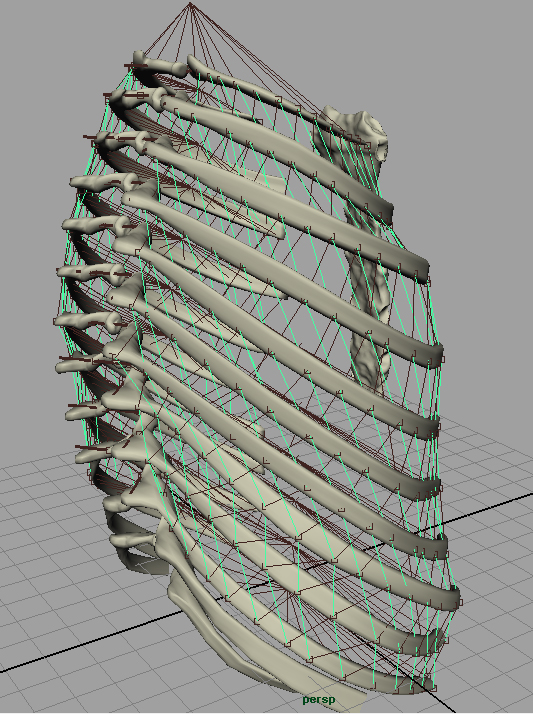
\includegraphics[width=0.45\textwidth]{pics/simu_externals}
\label{fig:simu_externals}
}
\subfigure[When activated, the internal intercostal muscles, in green, move the rib cage down.]{
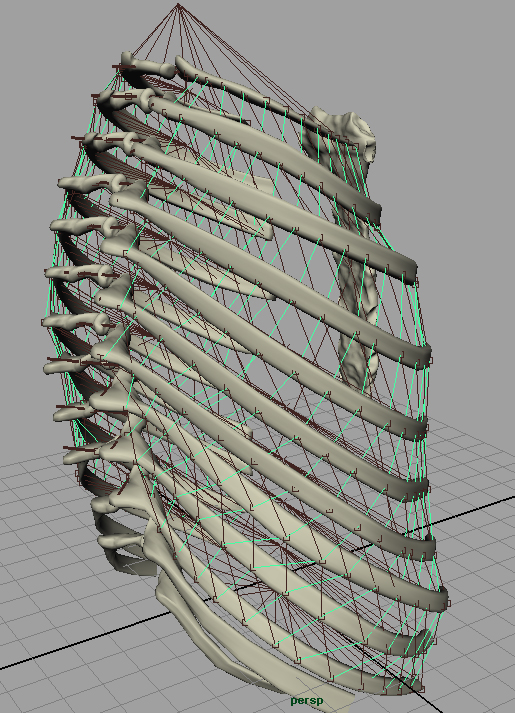
\includegraphics[width=0.45\textwidth]{pics/simu_internals}
\label{fig:simu_internals}
}
\caption[Simulation of the external intercostal the internal intercostal muscles]{\label{fig:simu_intercostals}\subref{fig:simu_externals} simulation of the external intercostal muscles and \subref{fig:simu_internals} the internal intercostal muscles.}
\end{figure}

\subsection{Scalene muscles}
The scalene muscles comprise three muscle heads that run from the transverse processes of the lower five cervical vertebrae to the upper surfaces of the first two ribs as shown in figure \ref{fig:scalene_muscles}. When activated, the scalene muscles produce an expansion of the upper rib cage. Although they have been considered to be `accessory' muscles of inspiration, electromyographic studies have established that they invariably contract during inspiration.

We modelled the scalene muscles with 12 spring elements linking the cervical vertebrae C6 to the first rib as shown in \ref{fig:simu_scalenes}.

\begin{figure}
\centering
\subfigure[The scalene muscles. Diagram taken from \cite{scalenemuscles2009}.]{
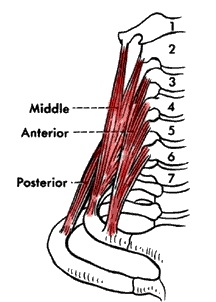
\includegraphics[width=0.3\textwidth]{pics/scalene_muscles}
\label{fig:scalene_muscles}
}
\subfigure[Simulation of the scalene muscles (in green).]{
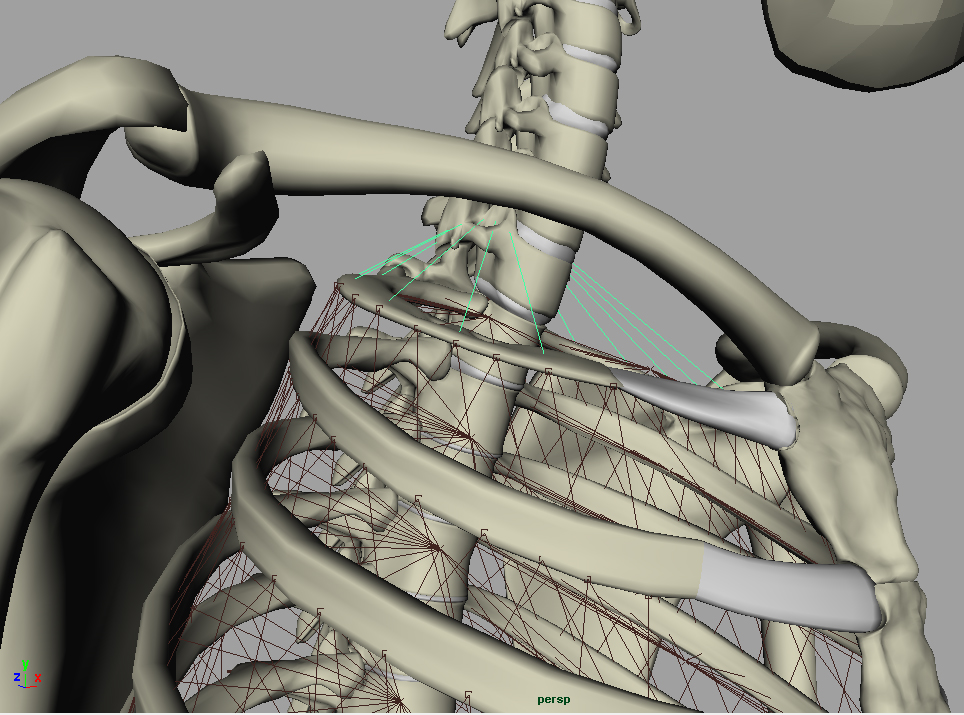
\includegraphics[width=0.6\textwidth]{pics/simu_scalenes}
\label{fig:simu_scalenes}
}
\caption[Comparison with the simulated scalene muscles]{\label{fig:scalenes}Comparison with the simulated scalene muscles.}
\end{figure}

% -------------------------------------------------------------
% Section
% -------------------------------------------------------------
\section{\label{sec:abdominal_cavity}Abdominal cavity}
The abdominal cavity is the cavity of the human body that holds the bulk of the viscera. It is located inferior to the thoracic cavity, and above the pelvic cavity. Organs of the abdominal cavity include the stomach, liver, gallbladder, spleen, pancreas, small intestine, kidneys, and large intestine.
The abdominal compartment contains between 100 and 300~mL of abdominal gas and the rest is incompressible. Therefore it can be reasonably considered as fully incompressible: any local inward displacement results in an equal outward displacement elsewhere in the compartment. Furthermore, the abdominal compartment is fixed dorsally to the spine, caudally to the pelvis and laterally with the iliac crests; which constrains the area of the abdominal compartment that can be displaced to the ventral abdominal wall and the diaphragm. The diaphragm itself is made of muscle fibres which insert onto the lower six ribs. During inspiration, when the diaphragm contracts the muscle fibres of the diaphragm shorten, and as a result the dome of the diaphragm goes down and the ventral abdominal wall moves outwards. This process expands the thoracic cavity along its cranio-caudal axis and displaces the abdominal viscera pushing the ventral abdominal wall outwards. As the diaphragm is connected to the lower six ribs, its contractions apply a force (called the insertional force) on these ribs in the cranial direction, lifting the ribs and rotating them outward such that the lower rib cage expands. Conversely, during relaxation when the abdominal muscles contract, the ventral abdominal wall moves inward and as a consequence, the diaphragm has a cranial motion up into the thoracic cavity. The mechanism is illustrated in figure \ref{fig:inspiration_expiration_diaphragm}. The diaphragm can shorten by 30 to 40~\% according to the authors of \cite{hamid2006phys}. From an anatomical point of view, there are four abdominal muscles: the rectus abdominis muscle (the most ventral, it runs caudally along the whole length of the abdominal wall), the transversus abdominis (the deepest of the muscles of the lateral abdominal wall), the external oblique muscle (the most superficial, it contracts caudally and medially) and the internal oblique muscle (see figure \ref{fig:abdominal_muscles}).

Posture also has an effect on breathing. For instance a change from the seated to the supine position increases the abdominal compliance, so the resistance from the abdominal contents to diaphragmatic descent is less effective and the forces applied by the diaphragm to expand the lower rib cage are reduced.

\begin{figure}
	\centering
	 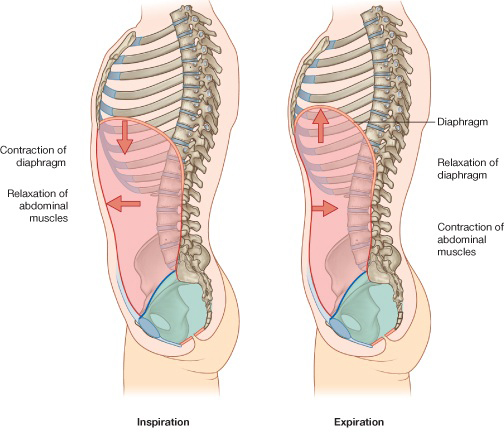
\includegraphics[scale=0.6]{pics/inspiration_expiration_diaphragm}
	 \caption[Sketch of how the abdomen assists in breathing]{\label{fig:inspiration_expiration_diaphragm}Sketch of how the abdomen assists in breathing. Diagram taken from \cite{drake2005gray}.}	
\end{figure}

\begin{figure}
	\centering
	 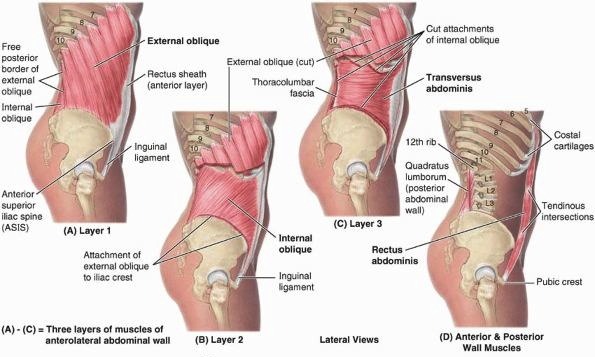
\includegraphics[scale=0.6]{pics/abdominal_muscles}
	\caption[The abdominal muscles]{\label{fig:abdominal_muscles}The abdominal muscles. Diagram taken from \cite{moore1992clinically}.}	
\end{figure}

We modelled the abdominal cavity by deformation of a polygonal sphere to produce the shape of the belly (see figure \ref{fig:simu_abdominal_cavity}). Then, we added the different muscle elements by attaching each muscle end to a vertex on the surface of the simulated cavity. The diaphragm was modelled with 500 spring muscles located at the top of the abdominal cavity (see figure \ref{fig:simu_diaphragm}). The four abdominal muscles were also modelled with spring muscles and 100 of them were used for the transversus abdominis (see figure \ref{fig:simu_transversus_abdominis}), 50 for the rectus abdominis (see figure \ref{fig:simu_rectus_abdominis}), 60 for the external obliques (see figure \ref{fig:simu_external_obliques}) and 60 for the internal obliques (see figure \ref{fig:simu_internal_obliques}).

\begin{figure}
\centering
\subfigure[Diaphragm.]{
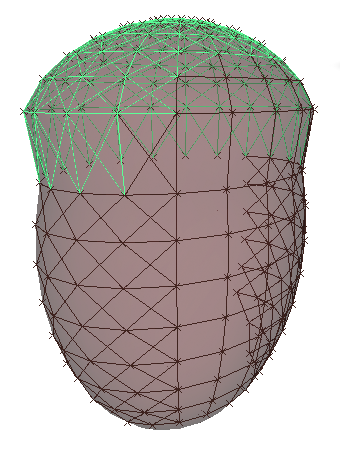
\includegraphics[width=0.3\textwidth]{pics/simu_diaphragm}
\label{fig:simu_diaphragm}
}
\subfigure[Transversus abdominis.]{
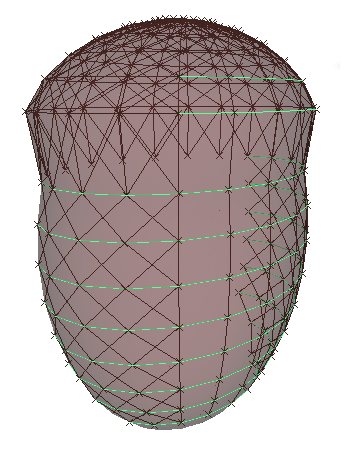
\includegraphics[width=0.3\textwidth]{pics/simu_transversus_abdominis}
\label{fig:simu_transversus_abdominis}
}
\subfigure[Rectus abdominis.]{
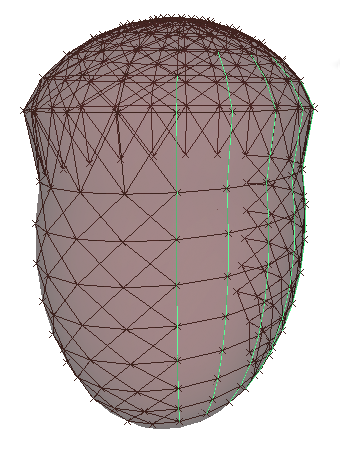
\includegraphics[width=0.3\textwidth]{pics/simu_rectus_abdominis}
\label{fig:simu_rectus_abdominis}
}
\subfigure[External obliques.]{
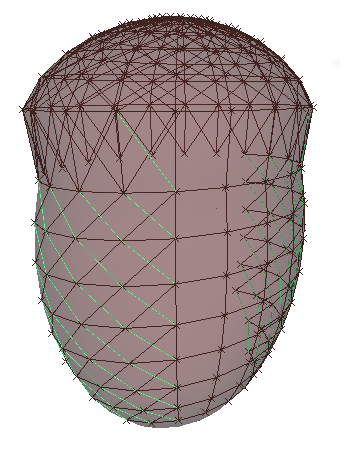
\includegraphics[width=0.3\textwidth]{pics/simu_external_obliques}
\label{fig:simu_external_obliques}
}
\subfigure[Internal obliques.]{
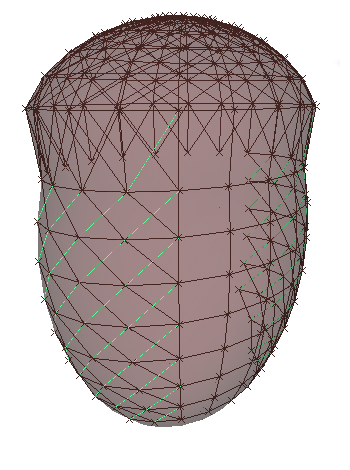
\includegraphics[width=0.3\textwidth]{pics/simu_internal_obliques}
\label{fig:simu_internal_obliques}
}
\caption[Simulation of the abdominal cavity muscles involved in breathing]{\label{fig:simu_abdominal_muscles}Simulation of the different muscles of the abdominal cavity involved in breathing.}
\end{figure}

\begin{figure}
	\centering
	 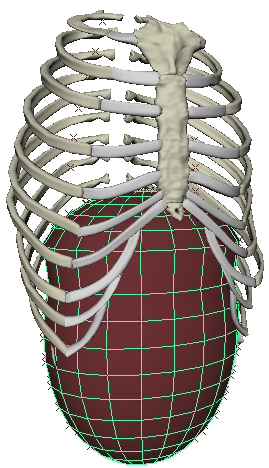
\includegraphics[scale=0.6]{pics/simu_abdominal_cavity}
	\caption[Simulation of the abdominal cavity]{\label{fig:simu_abdominal_cavity}Simulation of the abdominal cavity.}	
\end{figure}
% -------------------------------------------------------------
% Section
% -------------------------------------------------------------
\section{\label{sec:control_model}Control of the model}
The nature of the activation functions of the muscles involved in breathing are not currently well-defined, in either the medical or the animation communities. Nevertheless, some research is available in the literature and previous modelling attempts provide useful information concerning these activation functions.

As we are using spring muscle elements, we control the activation of each muscle by changing the contraction value as a time varying input parameter. Steady-state breathing is ideally periodic (usually 13--17 breaths per min in the average human \cite{slonim1987respiratory}); for that reason we naturally sought periodic input activations. Two major kinds of input have previously been proposed to control animation of physical muscle simulations: hand-crafted curves as Chen et al. \cite{chen1992pump} used in their model or sine functions as used by Terzopoulos et al. \cite{tu1994artificial} and the Breathe Easy model \cite{dilorenzo2009breathing}. In the latter, the authors experimented with both smooth and abrupt changes for the periodic contraction using simple sinusoid and step functions and concluded that sine functions created the desired response in steady-state breathing. As a consequence, we have also used different sine functions to stimulate the different muscles during steady state breathing.

Concerning the contraction of these muscles, Klute et al. \cite{klute2002artificial} found a contraction range from 0.7 to 1.2 for their artificial muscles. We used these data as limit constraints for our input functions.

The damping and stiffness parameters of the spring muscle elements as described in equation \ref{eq:spring_muscle}, were set to 1 for the intercostal and diaphragm muscles in order to have a system as close as possible to a \emph{critically damped} system (a system that converges to zero faster than any other without oscillations). These parameters were found empirically to avoid undesirable oscillations when the spring muscle elements were activated.

We activate a spring muscle element by changing its length $l(t)$ in time. For steady-state breathing, this length is modulated by a general sine function $r(t)$ in our simulation:

\begin{equation}l(t) = l_{0} \times r(t) \end{equation}
\begin{equation}\label{eq:sine_input}r(t) = \alpha - \frac{\beta}{2}\left(\sin\left(2 \pi f_{b} t + \phi\right) + 1\right) \end{equation}

where:
\begin{itemize}
\item[$\bullet$] $l_{0}$ is the rest length of the spring muscle element,
\item[$\bullet$] $\alpha \in [1, 1.2]$ is the offset value (i.e. the upper limit of function $r(t)$),
\item[$\bullet$] $\beta \in [0, 0.5]$ is the contraction value,
\item[$\bullet$] $f_{b}$ is the breath frequency,
\item[$\bullet$] $\phi$ is the phase.
\end{itemize}

The rest of this chapter describes the different activations we used for the muscles involved in chest and abdominal steady-state breathing.
	
\subsection{Chest breathing}
In chest breathing, three groups of muscles are active: the external intercostals, the internal intercostals and the scalene muscles. In contrast to other recent simulations \cite{dilorenzo2009breathing, lee2008biomechanical, veltkamp2009physiological}, we did not apply the same activation inputs for all the intercostal muscles. As shown in \ref{subsec:intercostal_mus}, the external intercostal muscles have an inspiratory moment which is the highest in the dorsal portion of the rib cage and decreases and reverses into an expiratory moment in the front of the rib cage and the internal intercostal muscles' moment mirrors that of the external intercostals (they have their highest expiratory moment in the front of the rib cage that decreases gradually along the rib in the dorsal direction to finally reverse to an inspiratory moment in the back part of the rib cage). For this reason, the activation functions in the external intercostal muscles were tuned such that the contraction value decreases along the rib from the head to the junction with the cartilage of the rib. The activation functions of the internal intercostals mirror the external ones.

The scalene muscles, located in the neck were grouped together.

Figure \ref{fig:simu_activations} shows the different activation functions $r(t)$ of the intercostals and the scalene muscles for one visually plausible breathing situation.

\subsection{Abdominal breathing}
We modelled the abdominal cavity as one incompressible volume as justified in section \ref{sec:abdominal_cavity}. During inspiration, the diaphragm (at the top of the abdominal cavity) contracts pushing the front of the belly outwards. During expiration, the diaphragm relaxes and goes up to its rest state, the abdominal muscles contribute in pushing the front of the belly inwards---even if they are not necessarily contracting. From a modelling perspective, the vertices of the polygonal sphere used to simulate the abdominal cavity are passive at the bottom and the back side, while those on the diaphragm, the lateral and front parts are active. To model the movement given the incompressibility constraint, we used a pressure approach as in \cite{dilorenzo2009breathing}. We assume that the pressure $P$ inside the cavity is determined by Hooke's law:

\begin{equation}P \propto \left(\frac{V_{0}}{V} - 1\right) \end{equation}
%\begin{equation}P = \max \left[ 0 , K \left(\frac{V_{0}}{V} - 1\right) \right]\end{equation}

where $V_{0}$ is the original volume and $V$ the current volume of the abdominal cavity. The coefficient of proportionality is called the `bulk volumetric modulus' and controls the substance's resistance to uniform compression. We found 0.3~Pa to be satisfactory. Since in our model the surface of the cavity is polygonal, being composed of triangles, the volume is calculated as the sum of tetrahedra (the base of each tetrahedron is a triangle of the surface and the apex a fixed point inside the polyhedron) inside the cavity. In order to make the active vertices of the front of the belly move outwards when the diaphragm contracts, for each active vertex, a force $\mathbf{F_{v}}$ proportional to the pressure $P$ times the area $A$ of the triangle attached to the vertex (this is defined by a specific ordering) is applied:

\begin{equation}\label{eq:pressure_force}\mathbf{F_{v}} = P \times \frac{A}{3}\mathbf{n} \end{equation}

where $\mathbf{n}$ is the direction vector of the force perpendicular to the triangle. The division by 3 accounts for the three vertices composing the triangle.

The abdominal muscles (see figure \ref{fig:abdominal_muscles}) can work autonomously, trying to preserve the pressure in the abdominal cavity by contracting to their rest lengths when they are stretched. However, they can also be activated to help the front of the belly move inwards more rapidly (some people and particularly sportsmen, actively use these muscles during expiration).

In the steady-breathing case, the diaphragm moves periodically and for that reason, we activate it with a sine function described in section \ref{sec:control_model}. An example of such an activation function for the diaphragm can be seen in figure \ref{fig:simu_activations}.

\begin{figure}
	\centering
	 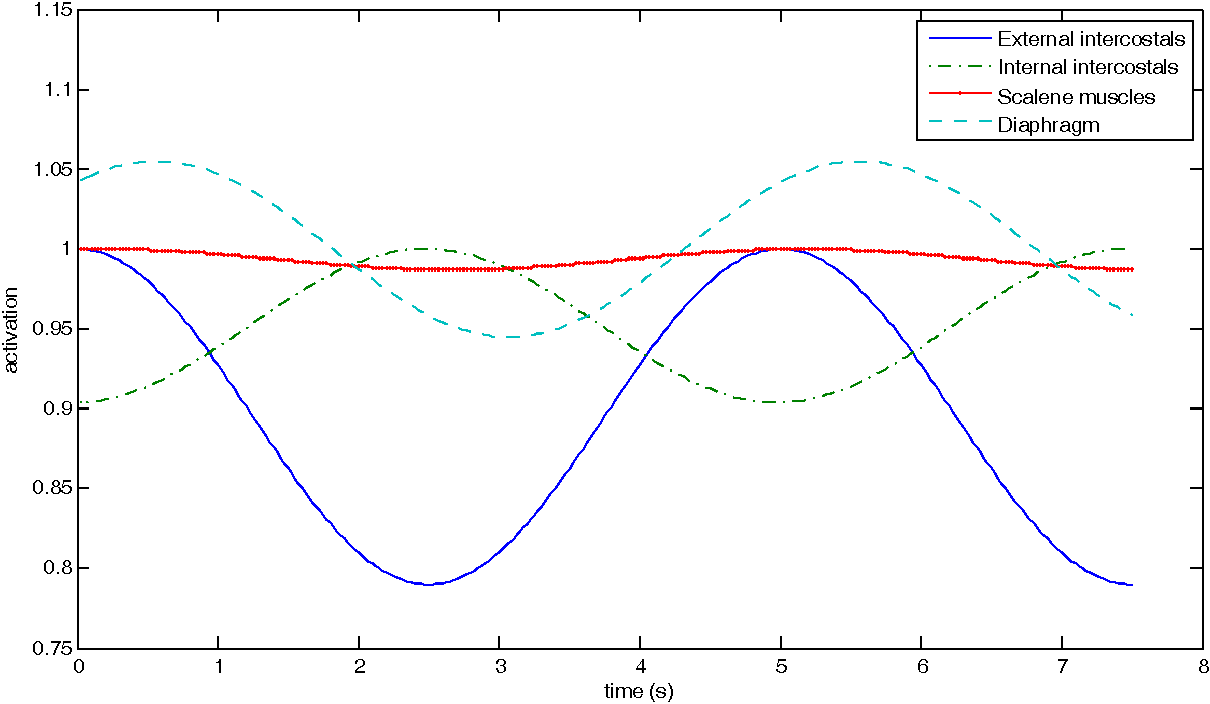
\includegraphics[width=1\textwidth]{pics/simu_act}
	\caption[Activation functions of the different muscles for a plausible simulation]{\label{fig:simu_activations}Activation functions of the different muscles for a plausible simulation.}	
\end{figure}